\documentclass{article}
\usepackage{amsmath, amsfonts, amsthm, amssymb}  

\usepackage{secdot}
\usepackage{epsfig}
\usepackage{cprotect}
\usepackage[T1]{fontenc}
\usepackage{epstopdf}
\usepackage{hyperref}
\usepackage{rotating}
\usepackage{graphicx}
\usepackage{caption}
\usepackage{subcaption}
\usepackage{multirow}
\usepackage{setspace}
\usepackage{array}
\usepackage{fancyhdr}
\usepackage{lastpage}
\usepackage[T1]{fontenc}

\usepackage{geometry}
\geometry{letterpaper, left=1in, right=1in, top=1in, bottom=1in}

\pagestyle{fancy}
\fancyhf{}
\rhead{\thepage/\pageref{LastPage}}
\lhead{OSU ECEN 2233 - Logic Design - Fall 2023}
\rfoot{\LaTeX}


% ----- Identifying Information -----------------------------------------------
\newcommand{\myassignment}{Lab 1: Using Testbenches More Effectively}
\newcommand{\myduedate}{Assigned: Monday 9/11 Due \textbf{Monday 9/25} (midnight)}
\newcommand{\myinstructor}{Instructor: James E. Stine, Jr., Rose Thompson}
% -----------------------------------------------------------------------------

\begin{document}
\begin{center}
  {\huge \myassignment} \\
  {\large \myduedate} \\
  \begin{flushright}
  \myinstructor \\
  \end{flushright}
\end{center}

\section{Introduction}

In Lab~$0$, you learned how to go through the procedure of
designing logic and the methodology in creating digital logic.  That
methodology is no different than what advanced engineers use at Apple
and AMD to create designs.  However, one of the differences is that experienced
engineers make good and ample use of testbenches.

To ramp our understanding of testbenches, this lab is about using
features of the testbenches to get used the process of
testbenches.  It is also about learning how testbenches work and using
them to simulate designs.  Fortunately, this laboratory is more about using the
simulation software than using the FPGA.  But, I want to emphasize
that testbenches are the key to making your digital design work
correctly.  They will also
be key to getting your future labs working.  Without good
testbenches, your implementations on your FPGA will \underline{never} work.
Therefore, I want to emphasize that this laboratory is vitally important for
your future labs and implementations and, more importantly, your career.

By the end of this laboratory, you should be
familiar with testbenches, how to create them, and what goes into them
to create good digital simulation.  The laboratory is really meant to
be an important process for future labs - therefore, please
try to understand everything about testbenches in this lab and how to
use them.

\subsection{Testbench}

Again, simulation is vital to making sure your hardware for any
architecture or
digital system works.  It is often the difference between something
that works and a bad product.  Therefore, it is
vital that for lab that you understand well how to construct a
testbench and use it to debug a more complicated design.
Engineers will typically spend days verifying their designs through
testbenches in hopes they catch all possible issues and anomalies.
Perhaps, you have owned a digital device that has behaved oddly
compared to what the owner's manual has indicated.  This occurred
because an engineer did not completely verify its specific operation.
Again, we plan on using ModelSim to help us this laboratory.

Although we will not discuss much of the theory here until later
in the semester, we will be using a clock in this laboratory.  A clock
is a synchronization signal usually created by an external device that
is accurate and provides an accurate synchronization of data
throughout your digital design.  In fact, as we will see later in the
semester, its one of the more important elements for a digital
device.  Your computer would be lost without the ability to keep
signals synchronized and the clock provides this as well as the
ability to move large amounts of data through your digital logic.

One of the things that gets a little confusing is that
SystemVerilog~\cite{5354441},
in general, is supposed to be for designing hardware.
However, they are also used many times for flushing
out topological designs
that are more behavioral.  This means you need some good way of
understanding how to get bits back and forth between systems. This is
really the job of the testbench.
%Without it, most simulations will
%not work correctly.

Although the book has a great chapter on this area (Chapter 4 of our
textbook), it is kind of difficult to follow when it comes to
testbenches.  This is because testbenches are typically best
understood by using it and not reading about them.  So, we will try to
understand more about testbenches and how they work in this
laboratory.  What is a testbench?

Testbenches are essential to HDL designs and they are not unique to
simulators.  They are part of the IEEE SystemVerilog
standard~\cite{5354441} and are typically
written in a behavioral manner.
Many testbench designs exist but using a
testbench that self-verifies the result is the best approach to create a
successful design. Therefore, it is encouraged that you utilize a
self-checking style or approach within your testbenches.
% Not sure what I was writing (jes)
%Although testbenches are
%usually written by the architect, this part of the lab a sample
%testbench is provided to you.  

Testbenches are written to be run with your simulation.  
The simulation environment runs a Tool Control Language (Tcl) file
called a \verb+DO+ file
that is basically a batch file for ModelSim that allows the simulation
to run regardless of a users set up.  A sample \verb+DO+ file is given
to you, but you should modify to make sure it runs your 
design and its appropriate testbench.  To run ModelSim with a
\verb+DO+ file, type the following command at a command prompt.
\begin{verbatim}
vsim -do file.do
\end{verbatim}
It is encouraged to consult your TA or the Internet to learn how to get to
the terminal in Microsoft Windows, so you can run your DO file
correctly.

\subsection{Basics of Testbench}

The testbench is another SystemVerilog file
that sits above, in hierarchy, your Verilog design that you wish to
test.  The testbench is written behaviorally and is \textbf{not}
synthesized!
It is only used to test your design and see if it works.  More
importantly, it is typically utilized with good known vectors that
comprise a good set of vectors that will assure your design will
work.  Normally, large digital designs are too difficult to test
exhaustively.  Therefore, good vectors that are symbolic of what would
normally be used in a real application are used to test whether your
design will work.

These test vectors are either generated with another program, a data
set of real-life applications, or generated within the testbench.  For
this laboratory, you will use vectors generated through the testbench
to test your design.  These \textit{known} test vectors are typically called
\textbf{golden vectors} as they represent the correct response 
for a given input.  For many applications,
specifications written by the Institute for Electronic and Electronics
Engineers (IEEE) or other specification/standard committees are used for
generating golden vectors.  However, for this laboratory we will
generate the golden vectors through our testbench.

Again, a test bench comprises a top-level SystemVerilog (SV) file that
instantiates the SV file one wishes to test.  This instantiated
design is called the device under test (DUT) or circuit under test
(CUT).  This can be represented visually as shown in Figure~\ref{tb.fig}
\begin{figure}
  \centering
  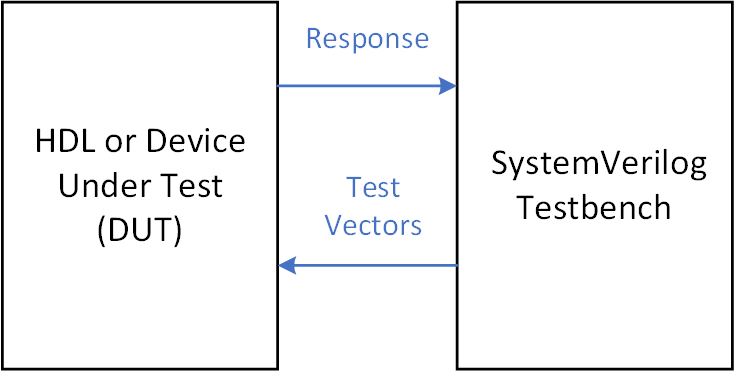
\includegraphics[scale=0.9]{Testbench.png}
  \caption{The TestBench Structure}
  \label{tb.fig}
\end{figure}

The basic structure of a testbench involves three distinct regions:
\begin{enumerate}
\item Internal declaration of inputs and outputs to the DUT as well as
  variables used for testing
\item Instantiating the DUT
\item Generating Test Vectors and Producing Output
\end{enumerate}
To create a testbench it is easiest to
instantiate the DUT or SV file you wish
to test as a basis for your testbench.  I typically copy over the SV
inputs, outputs, and module name I wish to test over to my testbench to create these
three parts to avoid misspellings and other issues.

The test vectors can be generated by an outside
program, however, they can be generated internally within
testbenches.  All good testbenches will have some mechanism to help
users test a design and demonstrate that the design is correct.
In addition, most
testbenches will also have some way of indicating that the SV vector
is correct.  This is called a self-validating testbench.  It makes
things easier and avoids issues related to sitting and looking at
thousands of vectors visually.  For example, suppose an output is
called \verb!Y_out! and you have a correct vector as
\verb!Y_correct!.  Inside your testbench, you can place some behavioral
construct within the SV that indicates the logic is bad or good and is
also an easy visual aid for indicating this event.  An
example would be as follows with a variable called \verb!Error!:
\begin{verbatim}
assign Error = Y_out != Y_correct;
\end{verbatim}
You are going to do a similar item with your design.

As the first laboratory demonstrated, making sure your SV works
\textbf{before} you go to implementation is vital.  As stated earlier
in this document many times, it is impossible to create an exhaustive
test for your design.  You could conceivably make an exhaustive test
for a smaller design, as in this laboratory, but normally this is not
possible.  For our work in this laboratory, we will create a $4$-bit
ripple-carry adder which is a good simple carry-propagate adder used
in many microcontrollers and simple adder structures.

\subsection{Testing Designs More Efficiently}

In Lab 0, we just used delay statements to test input vectors into our
design.  Although this worked acceptably for Lab 0, for larger designs, such
as in this laboratory, you have to figure an easier way to test more
vectors to save time.  For this design, we use the snippet of SV found in
Figure~\ref{test.fig}.

In this HDL, a clock is used to test the
design.  A clock is a periodic signal that uses a repetition of pulses
specifically used for synchronization.  In Figure~\ref{test.fig}, the clock
in the bottom half of figure.  The clock
is utilized to synchronize the data : that is, during the positive edge of
the clock (i.e., HIGH value), we assign a random signal to $A$ and $B$
and then on the negative edge of the clock (i.e., LOW value), the
values are displayed to a value called \verb!desc3!.

The value of \verb!desc3! is used to point to a file as seen by the
declaration within Figure~\ref{test.fig}.  All output designated by the
\verb!$fdisplay! keyword is sent to the output file.  The output
file is called \verb!rca.out! in this example, but can be any filename
you wish to use.  After you run, \verb!vsim -do file.do!, an output
file will be created that you can use to see if your design works
correctly.
As explained earlier, the output also compares the
true result to the computed result -- i.e., any output at the end of the
line which indicates an error.

The top part of Figure~\ref{test.fig} just declares variables for use
in this HDL snippet.  The \verb!integer! designation is just used in
testbenches to declare variables that are typically used for
\verb!for! or \verb!$fdisplay! statements.  The \verb!for! statement is
utilized specifically to randomly assign inputs for this test.  For
this snippet, Figure~\ref{test.fig} tests $128$ vectors, but can be
changed to any value.

The only caveat to the HDL in Figure~\ref{test.fig} is the
\verb!$finish! statement.  This item will end the simulation at the
time designated by the time within the delay statement. For this design, it ends at
time $1250$ ns.  
\begin{figure} [b!]
{\small
\begin{verbatim}
integer handle3;
integer desc3;
integer i;

initial
  begin
    handle3 = $fopen("rca.out");
    desc3 = handle3;	
    #1250 $finish;		
  end

initial
  begin
     for (i=0; i < 128; i=i+1)
       begin
          // Put vectors before beginning of clk
          @(posedge clk)
            begin
              A = $random;
              B = $random;
            end
          @(negedge clk)
            begin
     	      $fdisplay(desc3, "%h %h || %h | %h | %b", A, B, Sum, Sum_correct, (Sum == Sum_corr));
            end
       end // @(negedge clk)
  end 
\end{verbatim}
}
\caption{Sample HDL snippet to Test More Efficiently}
\label{test.fig}
\end{figure}


\subsection{Test Vehicle: Ripple Carry Adders}

Ripple carry adders (RCA) provide one of the simplest types of
carry-propagate adder designs.  Basically, a RCA is the method we
utilize to add two numbers
with paper and pencil.  It basically adds each bit together and then
passes the carry to each subsequent bit.  This type  of adder
is typically called a carry-propagate adder (CPA).
A CPA is an adder
where the carries are connected together to form a sum of two input
operands.
A $n$-bit RCA is formed by concatenating $n$ full adders (FA) similar
how I would add several numbers together on paper.  You
can use the full adder block you used from Lab 0 to help you with this
laboratory.  
The carry out from the $k^{th}$ FA is used as the carry in of 
the $(k + 1)^{th}$ FA, as shown in Figure~\ref{rca.fig}.  
%The main 
%advantage to this implementation is that it is efficient and easy to
%construct.
Unfortunately, since 
the connections for the carry-out depend on one another, 
most circuit implementations of RCAs
consume a significant amount of delay.  On the other hand, 
because the RCA implementation is straightforward
it can be easily implemented and
used for simple implementations and, more importantly, in courses
where time is of the essence.
\begin{figure} [tb]
\begin{center}
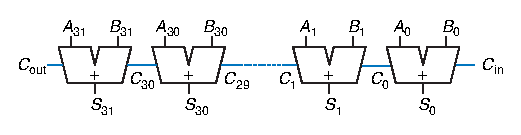
\includegraphics[scale=1.75]{f05-05-9780128000564.eps}
\end{center}
\caption{$32$-bit Ripple-Carry Adder (RCA) Implementation from our Text~\cite{ddca-riscv}.}
\label{rca.fig}
\end{figure}

In order to create a RCA, you will have to use hierarchy similar to
what you will do for the testbench.  You will have to instantiate four
($4$) full adder (FA) blocks from Lab 0 to create your $4$-bit
ripple-carry adder.  There are more advanced SV features that
allow one to automate repeated instantiations (e.g., for-generate
blocks), but we will just instantiate our full adder $4$ times in this
laboratory.

To create a good known golden vector for your adder, you will have to
use a behavior construct to help you compute the correct sum or
result.  Although
behavior constructs in SV have gotten much better over the
years, they still have a ways to go for some pieces of digital logic.
Until you get comfortable designing digital logic structurally, it is
best to use only the behavior HDL blocks we recommend.  To compute a
known sum to compare versus your output, you should
use this behavior construct within your SV testbench:
\begin{verbatim}
assign Sum_correct = A + B + Cin
\end{verbatim}
In this example, it is important to note the use of the $+$ operator
is not an OR statement.  Interestingly, these operators
are rather awesome in that they actually synthesize very good
implementations.  However, for this laboratory your job is to use this
behavior construct to compare the result of your $4$-bit RCA is
correct.

\section{Implementation}

To get started there are a couple of downloads that will help you
get started.  All of these files are found within a zip file on Canvas
called \verb!lab1.zip!.
The first item is a complete SV file, testbench and DO
file from Lab 0 you can use as a template for your test (i.e., the
silly SV files).   
Second, there is a zip
file of a demo program that is slightly different than Lab 0.  In your
new demo program, it contains logic to output a $4$-bit value to a
$7$-segment display.  
%The demo program is similar to your Lab 0 demo program in that you need
%to also instantiate your RCA design (i.e., \textbf{without} the
%testbench).
It is important to state that you should not include your testbench in
your implementation. The testbench is only used to verify your design
works \textbf{before} you synthesize and implement it.

Once you design the SV of your $4$-bit ripple-carry adder
and test it thoroughly, implement it on the
FPGA board.  This should be fairly easy if you use the demo program
(i.e., zipped file) to instantiate the design of your RCA.
That is, once inside Vivado, open the unzipped file by navigating
through \verb!File->Project->Open! and opening the \verb!Lab1.xpr!
project.  Once the project has opened, go to the \verb!top_demo.sv!
source by double-clicking the \verb!top_demo!
design.  You can instantiate your RCA in the \verb!top_demo.sv! but
may need to add your SV files to your project to get it to synthesize
correctly.
Please ask your TA if you are unsure
how to add files to your \verb!Lab1.xpr! project.

\subsection{Seven-Segment Display}

If you examine your textbook in Example $2.10$~\cite{ddca-riscv},
you can see some
information on a $7$-segment display.
A seven-segment display decoder takes a $4$-bit data input
\verb!D[3:0]! and produces seven outputs to control light-emitting
diodes (LEDs) to display a digit.
Some seven segment display implementations, such as ours in this
laboratory, will display the output from $0$ to $F$.  However, some
may only output $0$ to $9$ in applications where users do not know
what a hexadecimal output are.
The seven outputs are often
called segments $a$ through $g$, or Sa–Sg, as defined in Figure~$2.47$ in
your textbook~\cite{ddca-riscv}. The
digits are shown in Figure~$2.48$ in your textbook~\cite{ddca-riscv}.

For this implementation, the $7$-segment display implementation is
already set up for you.  You just have to send the $4$-bit value to
that digital instantiated part and it will display correctly on your
DSDB board.  For this laboratory, you want to send both $A$ and $B$
(i.e., both input operands) to your $7$-segment display as well the
sum.  Since there are four $7$-segment displays on your DSDB board,
please use two $7$-segment
displays for your $5$-bit sum (i.e., since $c_{out}$
will be the \verb!sum[5]!).  To use the $7$-segment display, just
assign a value to one of the inputs within the \verb!segment_driver!
instantiation for
\verb!digit0! through \verb!digit3!.  You should make sure that any value
given to this instantiation is a $4$-bit quantity.  You can also experiment
with it to see known outputs - for example, you can see one of the
values in
Figure~\ref{demo.fig} is the value \verb!0xF! or \verb!4'b1111!
given to \verb!digit3!.
\begin{figure}
{\small
\begin{verbatim}
 // 7-segment display
  segment_driver driver(
  .clk(smol_clk),
  .rst(btn[3]),
  .digit0(sw[3:0]),
  .digit1(4'b0111),
  .digit2(sw[7:4]),
  .digit3(4'b1111),
  .decimals({1'b0, btn[2:0]}),
  .segment_cathodes({sseg_dp, sseg_cg, sseg_cf, sseg_ce, sseg_cd, sseg_cc, sseg_cb, sseg_ca}),
  .digit_anodes(sseg_an)
  );
\end{verbatim}
}
\cprotect\caption{Instantiation of $7$-segment display in
  \verb!Lab1.zip! Demo program}
\label{demo.fig}
\end{figure}

\subsection{Power, Performance and Area (PPA)}

As with the first laboratory, you should discuss your
Power, Performance and Area (PPA)
analysis.  You should document in your report how much PPA is utilized
for your final design.  Similar to the previous laboratory, please report
the total number of ``slices'' used for your design.  We will expand
your PPA for power and performance in later labs.

\section{What to design?}

Similar to Lab 0, you will be using the DSDB board.
For this laboratory, you will also use the slide switches (i.e,
\verb!btn[7:0]!) to select the
inputs.  You might need to use the push buttons (i.e., \verb!sw[3:0]!
to indicate a carry in signal), the LEDs on board to help in
debugging, and of course the $7$-segment display
explained in the previous Section.

The following are items will be needed to complete this laboratory:
\begin{enumerate}
  \item Using the full adder from Lab 0, design a $4$-bit structural
    version of a ripple carry
    adder to add two $4$-bit input operands and a $1$-bit Carry In
    signal.  You can read more about the ripple-carry adders in
    Chapter~$5$ of your textbook.  Although we did not discuss the
    ripple-carry adder (RCA) in depth,
    the idea should be easy to understand from
    Figure~\ref{rca.fig} above and Figure~$5.5$ in your text.  What
    you should do is instantiate $4$ full adders and connect them
    appropriately.  
    \item Create a testbench from the \verb!silly_tb.sv! testbench from
      Lab 0 to test your RCA.  
    \item Integrate a self-validating structure into your testbench so
      that it checks the answer automatically.  Test, at least, $175$
      different vectors and demonstrate that the sum is indeed
      correct.  That way, it
      should be easy to see if a signal is asserted when an error
      occurs.
      It should also be relatively easy to test all vectors and
      relax knowing that you have exhausitively verified your design too.
    \item Once your RCA works, implement your design on the RCA
      using the demo program from \verb!Lab1.zip!.  Your design should
      display the input operands (i.e., $A$ and $B$) and the final
      sum on the $7$-segment display.
\end{enumerate}

\subsection{Importance}

Although this laboratory is somewhat minimal compared to previous and
future labs, the topics are of extreme importance for digital design.
Verification dominates many products today and having good testbenches
is vital, even in mixed-signal designs (i.e., analog and digital
designs).  I have heard hearsay from some companies that have told me
they spend more than  $70\%$ of their design time on verification.
Therefore, I implore you to learn as much as you can about
testbenches and ask questions when possible.  It will also pay
\textbf{huge} dividends and may even shorten your development time
in later labs if you can understand
verification with testbenches well.

\subsection{Handin}

You should electronically hand in your HDL (all files that you want
us to see) into Canvas.
You should also take a printout of your waveform 
from your ModelSim simulation.  
Only one of your team members should upload
the files and/or lab report. Please contact
the instructor James Stine (james.stine@okstate.edu) 
for more help.  Your code should be
readable and well-documented. In addition, please turn in additional
test cases or any other added item that you used. 
Please also remember to document everything in your Lab Report using
the information found in the Grading Rubric.

\subsection{Extra Credit}

You will use the four $7$-segment displays on your DSDB board to help
highlight the input operands and your sum.  However, the current
$7$-segment display that is instantiated in Figure~\ref{demo.fig} is
written to display hexadecimal numbers.  You could add another
instantiated design between your RCA and the \verb!segment_driver! to
convert the output into decimal.  This is not very hard, but might
be a little tricky.  Early computers did this with something called
packed Binary-Coded Decimal (BCD) and I encourage you to look up this
format to help you (see Exercise 1.64 in~\cite{ddca-riscv} as well as
the Wikipedia entry for
BCD~\footnote{\url{https://en.wikipedia.org/wiki/Binary-coded_decimal}}).
There is also an excellent journal that discusses information on this too
and is included in your repository~\cite{1453497}.
Although the implementation is a little tricky it
is not terribly difficult to implement.

\bibliographystyle{IEEEtran}
\bibliography{IEEEabrv,lab1}

\end{document}
